%   ================================================================================
%   thesis.tex
%   ================================================================================
%   College of Technology Thesis Template - 2010-05-06 - Robert S. Cutler (rcutler@purdue.edu)
%     Updated on 2012-04-03 by Jason St. John (jstjohn@purdue.edu)
%     This template has been tested using TeX Live 2012
%
%   Based on the LaTeX thesis template file:
%       thesis.tex  2011-07-01  Mark Senn  https://engineering.purdue.edu/~mark
%   ================================================================================
%
%  This is the thesis ``root file''.
%
%  To print the final copy of your thesis put a '%'
%  in front of the \includeonly command and type
%  (from page 71 of _LaTeX User's Guide and Reference Manual_, 2nd edition):
%      latex thesis
%      bibtex thesis
%      latex thesis
%      latex thesis
%
%  In "Reference:" listings below:
%      KEY  MEANING
%      TM   ``A Manual for the Preparation of Graduate Theses'',
%             seventh revised edition, The Graduate School, 2006.
%             http://www2.itap.purdue.edu/gradschool//Publications/graduate-thesis-manual.pdf
%      PU   ``A Manual for the Preparation of Graduate Theses'',
%           The Graduate School, Purdue University, 1996.
%           http://www2.itap.purdue.edu/gradschool//Publications/graduate-thesis-manual.pdf
%
%  Search for "CHANGE" below and change things as necessary.
%  I recommend putting "%%" before any existing lines that
%  need to be changed and adding your new line(s) immediately
%  below the existing lines.
%

% See https://engineering.purdue.edu/~mark/puthesis/#Options
% for documentclass options.
%     'thesisproposal' is a new type added by Robert S. Cutler
%     'dissertationproposal' is a new type added by Robert S. Cutler
%     'nochapterblankpages' removes the requirement that chapters must start on odd-numbered pages
%     'uglyheadings' is the correct style for CoT
% CHANGE NEXT LINE?
\documentclass[tech,thesisproposal,apacite,nochapterblankpages,uglyheadings]{puthesis-cot}

%   ------------------------------------------------------------------------------------------------------------------------
%   \usepackage{indentfirst}
%   
%       Ensures that the first paragraph after a \section or \subsection tag is indented
%       properly.  (All other paragraphs are automatically indented properly.)
%
%   \newcommand{\ip}{\mbox{}\indent}
%       Unfortunately, the previous package does not work with the first paragraph 
%       after a \subsubsection tag.  Put the tag \ip after a \subsubsection tag to indent the
%       first paragraph after the \subsubsection tag.
%   ------------------------------------------------------------------------------------------------------------------------
\usepackage{indentfirst}
\newcommand{\ip}{\mbox{}\indent}


% Define "align" environment used in demo-mathematics.tex.
% CHANGE NEXT LINE?
\usepackage{amsmath}

% Define "multicols" environment environment used in demo-multicols.tex.
% CHANGE NEXT LINE?
\usepackage{multicol}

% Define "subfigure" environment used in "demo-figure.tex".
% CHANGE NEXT LINE?
\usepackage{subfigure}

% Title of thesis (used on cover and in abstract).
% The title shown must be the full, official title of the
% thesis.  Superscripts and subscripts are not permitted in
% the title.
% Reference: TM 26.
% Use \title{Put Title Here} for a one-line title.
% Use \\ to separate lines.
% Put % at the end of the last line to avoid getting an extra space
% in the abstract.
% There are two forms of title: one line or more than one line.
% There are examples of both below.
% Only use one \title.
% CHANGE NEXT FOUR LINES.
\title{An Example Thesis Done with \LaTeX}
\title{%
  An Example Thesis Done with \LaTeX\\
  with a Very Long Title in the\\
  College of Technology%
}

% First author name with first name first is used for cover.
% Second author name with last name first is used for abstract.
% Your full name as it appears in the University records appears
% on the cover.
% Reference: TM 26, 29.
% There are two forms of author, with and without initials.
% There are examples of both below.
% Only use one \author line.
%
% Template:
% \author{Firstname M. Lastname}{Lastname, Firstname M.}
%
% CHANGE NEXT TWO LINES.
\author{Mark Senn}{Senn, Mark}
\author{Mark D. Senn}{Senn, Mark D.}

% First is long title of degree (used on cover).
% Second is abbreviation for degree (used in abstract).
% Third is the month the degree was (will be) awarded (used on cover
% and abstract).
% Last is the year the degree was (will be) awarded (used on cover
% and abstract).
% The degree title for all doctoral candidates is ``Doctor of Philosophy.''
% The precise degree names for master's candidates appear in the list of
% ``Degrees Offered'' in the Graduate School bulletin.
% The date is the month and year that the degree is actually awarded.
% (If you have registered for ``degree only,'' revise the thesis title
% page to reflect the new date on which the degree is to be awarded.)
% Reference: TM 26--27, 30.
% Only use one \pudegree line.
% CHANGE NEXT LINE?
\pudegree{Doctor of Philosophy}{Ph.D.}{May}{2012}
\pudegree{Master of Science}{M.S.}{May}{2012}

% Major professor (used in abstract).
% Use, for example:
%     \majorprof{John Q. Professor}
%     \majorprofs{John Q. Professor and Thomas R. Jones}
%     \majorprofs{John Q. Professor, Thomas R. Jones, and David S. Smith}
% depending on the number of major professors you have.
% CHANGE NEXT LINE.
\majorprof{James L. Mohler}

% Campus (used only on cover)
% Use one of the following:
%     Fort Wayne
%     Hammond
%     Indianapolis
%     West Lafayette
%     Westville
% Reference: TM 27.
% CHANGE NEXT LINE?
\campus{West Lafayette}

% My command definitions not specific to my thesis.
% CHANGE NEXT LINE?
%
%  mydefs.tex  2007-03-19  Mark Senn  https://engineering.purdue.edu/~mark
%
%  Command definitions that can be used in all documents that have
%      %
%  mydefs.tex  2007-03-19  Mark Senn  https://engineering.purdue.edu/~mark
%
%  Command definitions that can be used in all documents that have
%      %
%  mydefs.tex  2007-03-19  Mark Senn  https://engineering.purdue.edu/~mark
%
%  Command definitions that can be used in all documents that have
%      \input{mydefs}
%

% CHANGE NEXT 3 LINES?
% Define \be and \ee to start and end the equation environment.
\newcommand{\be}{\begin{equation}}
\newcommand{\ee}{\end{equation}}

% CHANGE NEXT 12 LINES?
% Define \Repeat so, for example,
%     \Repeat{whatever}{10}
% is the same as typing whatever 10 times.
\newcount{\myi}
\newcommand{\Repeat}[2]{%
    \myi=0
    \loop
        \ifnum\myi<#2
        #1
        \advance\myi by 1
    \repeat
}

% CHANGE NEXT 3 LINES?
% Make "\Sum ab" or "\Sum{a}{b}" do "\sum_{a}^{b}".
% This can only be used when in math mode.
\newcommand\Sum[2]{\sum_{#1}^{#2}}

% CHANGE NEXT 4 LINES?
% Make "\xn" do "$x_n$".
% Because this definition contains the "$" to go into math mode
% this definition must be used when not in math mode.
\newcommand{\xn}{$x_n$}

% CHANGE NEXT 5 LINES?
% Since \xn is already defined we must use \renewcommand to redefine it.
% Normally you would not have the above definition for \xn in this file
% if you were just going to override it later.
% The \ensuremath goes into math mode if not already in math mode.
\renewcommand{\xn}{\ensuremath{x_n}}


%

% CHANGE NEXT 3 LINES?
% Define \be and \ee to start and end the equation environment.
\newcommand{\be}{\begin{equation}}
\newcommand{\ee}{\end{equation}}

% CHANGE NEXT 12 LINES?
% Define \Repeat so, for example,
%     \Repeat{whatever}{10}
% is the same as typing whatever 10 times.
\newcount{\myi}
\newcommand{\Repeat}[2]{%
    \myi=0
    \loop
        \ifnum\myi<#2
        #1
        \advance\myi by 1
    \repeat
}

% CHANGE NEXT 3 LINES?
% Make "\Sum ab" or "\Sum{a}{b}" do "\sum_{a}^{b}".
% This can only be used when in math mode.
\newcommand\Sum[2]{\sum_{#1}^{#2}}

% CHANGE NEXT 4 LINES?
% Make "\xn" do "$x_n$".
% Because this definition contains the "$" to go into math mode
% this definition must be used when not in math mode.
\newcommand{\xn}{$x_n$}

% CHANGE NEXT 5 LINES?
% Since \xn is already defined we must use \renewcommand to redefine it.
% Normally you would not have the above definition for \xn in this file
% if you were just going to override it later.
% The \ensuremath goes into math mode if not already in math mode.
\renewcommand{\xn}{\ensuremath{x_n}}


%

% CHANGE NEXT 3 LINES?
% Define \be and \ee to start and end the equation environment.
\newcommand{\be}{\begin{equation}}
\newcommand{\ee}{\end{equation}}

% CHANGE NEXT 12 LINES?
% Define \Repeat so, for example,
%     \Repeat{whatever}{10}
% is the same as typing whatever 10 times.
\newcount{\myi}
\newcommand{\Repeat}[2]{%
    \myi=0
    \loop
        \ifnum\myi<#2
        #1
        \advance\myi by 1
    \repeat
}

% CHANGE NEXT 3 LINES?
% Make "\Sum ab" or "\Sum{a}{b}" do "\sum_{a}^{b}".
% This can only be used when in math mode.
\newcommand\Sum[2]{\sum_{#1}^{#2}}

% CHANGE NEXT 4 LINES?
% Make "\xn" do "$x_n$".
% Because this definition contains the "$" to go into math mode
% this definition must be used when not in math mode.
\newcommand{\xn}{$x_n$}

% CHANGE NEXT 5 LINES?
% Since \xn is already defined we must use \renewcommand to redefine it.
% Normally you would not have the above definition for \xn in this file
% if you were just going to override it later.
% The \ensuremath goes into math mode if not already in math mode.
\renewcommand{\xn}{\ensuremath{x_n}}




% My command definitions specific to my thesis.

% CHANGE NEXT LINE TWO LINES?
% Set things up so \margins will show where the margins on the page are.
\newcommand{\margins}{\Repeat{Show where the margins for the page are.}{4}}

% CHANGE NEXT TWO LINES?
% Let typing "\en" be exactly the same as typing "\ensuremath". 
\let\en=\ensuremath

% CHANGE NEXT FIVE LINES?
% Define a \ve command with two arguments, so if it called with
%     \ve an
% it will expand to
%     {\en{a_1},~\en{a_2},\ \ldots,~\en{a_{n}}}
\newcommand{\ve}[2]{\en{#1_1},~\en{#1_2},\ \ldots,~\en{#1_{#2}}}


% To LaTeX only some parts of your thesis put the
% names of the parts to include here.  For example,
% \includeonly{front} would only process front.tex.
% \includeonly{front,introduction} would only process
% front.tex and introduction.tex.
% To print the final copy of your thesis put a '%'
% in front of the \includeonly command and run LaTeX
% three times to make sure that all cross-references
% are correct.  Then run BibTeX once and LaTeX twice
% more.
% CHANGE NEXT LINE?
%\includeonly{front,introduction}

\begin{document}

% Start a new volume for your thesis.  All theses must have at least one
% volume.  If your thesis is too long to fit in one binder put another
% "\volume" between chapters below.
\volume

% Front matter (dedication, etc.).
%
%  revised  front.tex  2011-09-02  Mark Senn  https://engineering.purdue.edu/~mark
%  created  front.tex  2003-06-02  Mark Senn  https://engineering.purdue.edu/~mark
%
%  This is ``front matter'' for the thesis.
%
%  Regarding ``References'' below:
%      KEY    MEANING
%      PU     ``A Manual for the Preparation of Graduate Theses'',
%             The Graduate School, Purdue University, 1996.
%      TCMOS  The Chicago Manual of Style, Edition 14.
%      WNNCD  Webster's Ninth New Collegiate Dictionary.
%
%  Lines marked with "%%" may need to be changed.
%

  % Dedication page is optional.
  % A name and often a message in tribute to a person or cause.
  % References: PU 15, WNNCD 332.
\begin{dedication}
  This is the optional dedication.
  The dedication usually consists of a name or cause as in:\\
  Dedicated to my grandmother.
\end{dedication}

  % Acknowledgements page is optional but most theses include
  % a brief statement of apreciation or recognition of special
  % assistance.
  % Reference: PU 16.
\begin{acknowledgments}
  This is the optional acknowledgments section.
  Most theses include brief statements of appreciation or recognition of special assistance as in:

  I wish to gratefully acknowledge my thesis committee for their insightful comments and guidance and my family for their support and encouragement.
\end{acknowledgments}

  % The preface is optional.
  % References: PU 16, TCMOS 1.49, WNNCD 927.
\begin{preface}
  This is the optional preface.

  A preface includes introductory remarks here regarding reasons for undertaking this work and method of research.

  Since everyone knows you're writing this document to get your degree, don't put that here.
  If your research was done to solve a problem that came up in industry, you may want to put that here.

  If not obvious from the rest of your thesis, you may want to describe your method of research here.

  Acknowledgements go in the ``Acknowledgments'' section and do not belong here.
\end{preface}

  % The Table of Contents is required.
  % The Table of Contents will be automatically created for you
  % using information you supply in
  %     \chapter
  %     \section
  %     \subsection
  %     \subsubsection
  % commands.
  % Reference: PU 16.
\tableofcontents

  % If your thesis has tables, a list of tables is required.
  % The List of Tables will be automatically created for you using
  % information you supply in
  %     \begin{table} ... \end{table}
  % environments.
  % Reference: PU 16.
\listoftables

  % If your thesis has figures, a list of figures is required.
  % The List of Figures will be automatically created for you using
  % information you supply in
  %     \begin{figure} ... \end{figure}
  % environments.
  % Reference: PU 16.
\listoffigures

  % List of Symbols is optional.
  % Reference: PU 17.
\begin{symbols}
  $m$& mass\cr
  $v$& velocity\cr
\end{symbols}

  % List of Abbreviations is optional.
  % Reference: PU 17.
\begin{abbreviations}
  abbr& abbreviation\cr
  bcf& billion cubic feet\cr
  BMOC& big man on campus\cr
  AT& Aviation Technology\cr
  BCM& Building and Contruction Management\cr
  CGT& Computer Graphics Technology\cr
  CIT& Computer and Information Technology\cr
  CoT& College of Technology\cr
  ECET& Electrical and Computer Engineering Technology\cr
  MET& Mechanical Engineering Technology\cr
  TLI& Technology Leadership and Innovation\cr
\end{abbreviations}

  % Nomenclature is optional.
  % Reference: PU 17.
\begin{nomenclature}
  Alanine& 2-Aminopropanoic acid\cr
  Valine& 2-Amino-3-methylbutanoic acid\cr
\end{nomenclature}

  % Glossary is optional
  % Reference: PU 17.
\begin{glossary}
  chair& the person in charge of a meeting or organization\cr
  chick& female, usually young\cr
  dude& male, usually young\cr
\end{glossary}

  % Abstract is required.
  % Note that the information for the first paragraph of the output
  % doesn't need to be input here...it is put in automatically from
  % information you supplied earlier using \title, \author, \degree,
  % and \majorprof.
  % Reference: PU 17.
  %
  % The abstract is required for theses and dissertations. It is
  % optional for thesis proposals and dissertation proposals. 
\begin{abstract}
  The first paragraph must contain your name as it appears on the title page but with the last name first, the abbreviation of the degree title, the name of the institution granting the degree, the month and year the degree is awarded, the title of the thesis, and the name(s) of your major professor(s).
  This paragraph is automatically generated by \LaTeX based on the information you provided in thesis.tex.
  Follow the first paragraph with a statement of your thesis problem, a brief exposition of the research and a condensed summary of your findings.
\end{abstract}


% Put chapter \include commands here.
% CHANGE \include{...} COMMANDS BELOW?
%
%  revised  introduction.tex  2012-04-26  Jason St. John <jstjohn@purdue.edu>
%  introduction.tex  2012-01-18  Mark Senn  https://engineering.purdue.edu/~mark
%
%  This is the introduction chapter for a simple, example thesis.
%


\chapter{Introduction}
% You should include a few sentences to introduce your thesis before transitioning
% into the scope, significance, etc. sections. This ensures that (1) the reader has
% some narrative introducing the thesis before jumping into the various sections and
% (2) that the first section heading is separated from the chapter heading with text.

This is a sample introduction that you should change to fit your thesis topic.
This is another sentence in the very beginnings of the introduction.
Note that the first paragraph after a heading is not indented.

This is a sentence.
This is a sentence.

\section{Scope}

This paper critically examines why you should write your thesis using \LaTeX in the College of Technology.

This is a sentence.


\section{Significance}

This is a significant sentence.


\section{Research Question}

What is your research question?


\section{Assumptions}

The assumptions for this study include:
\begin{itemize}
\item first
\item second
\item third
\end{itemize}


\section{Limitations}

The limitations for this study include:
\begin{itemize}
\item first
\item second
\item third
\end{itemize}


\section{Delimitations}

The delimitations for this study include:
\begin{itemize}
\item first
\item second
\item third
\end{itemize}


\section{Definitions}
In the broader context of thesis writing, we define the following terms:
\begin{italicdesc}
\item[\LaTeX:] A typesetting application that makes really impressive looking documents
\item[Purdue University:] (commonly: \textit{Purdue}) A public university founded in 1869
\item[Boilermakers:] Purdue University's official mascot
\end{italicdesc}


\section{Other Stuff}

\subsection{Thesis}

A long research paper used to satisfy requirements for a Master's Degree.


\subsection{Thesis Proposal}

The proposal for the thesis.


\subsection{Dissertation}

A longer research paper used to satisfy requirements for the Doctor of Philosophy (Ph.D.) degree.


\subsection{Dissertation Proposal}

The proposal for the dissertation.


\section{Summary}

This chapter provided the scope, significance, research question, assumptions, limitations, delimitations, definitions, and other background information for the research project.
The next chapter provides a review of the literature relevant to ``your thesis''.



% The literature review
% The placement of this section may be incorrect!
%	================================================================================
%	literaturereview.tex
%	================================================================================
%	College of Technology Thesis Template - 2010-05-06 - Robert S. Cutler (rcutler@purdue.edu)
%     Updated on 2012-04-16 by Jason St. John (jstjohn@purdue.edu)
%
%	Based on the LaTeX thesis template file:
%  		introduction.tex  2011-09-02  Mark Senn  https://engineering.purdue.edu/~mark
%	================================================================================

\chapter{Review of Relevant Literature}
% Do not include a heading for the introduction section

This chapter provides a review of the literature relevant to something awesome (e.g. your thesis!).

\section{Section}
A section...


\subsection{Subsection}
A subsection...


\subsubsection{Subsubsection}
\ip
A subsubsection...  (Note the use of the \\ip command in the source text to handle indentation correction.)


\section{Summary}

This chapter provided a review of the literature relevant to something awesome.
The next chapter provides the framework and methodology to be used in the research project.


% The methodology section
% The placement of this section may be incorrect!
%
%  This generally targets a quantitative study, so adjust this chapter as appropriate
%  for qualitative or mixed methods studies.
%

\chapter{Framework and Methodology}
% Do not include a heading for the introduction section. In other words, leave the
% following in place or replace it if you want, but do not add \section{Introduction}
% or something similar.

This chapter provides the framework and methodology to be used in the research study.

\section{Study Design}

This study blah, blah, blah...


\section{Unit \& Sampling}

The following sections will discuss the hypotheses, population, sample(s), variables, and the measure for success.

\subsection{Hypotheses}

More blah, blah, blah...

The hypotheses for this study are the following:

\begin{quote}
H\textsubscript{0}: This is the null hypothesis.

H\textsubscript{$\alpha$}: This is an example alternate hypothesis.
\end{quote}


\subsection{Population}

This discusses the population.


\subsection{Sample}

This discusses the sample.


\subsection{Variables}

This discusses the variables.


\subsection{Measure for Success}

This discusses the criterion for what constitutes a ``success'' (i.e. what criterion are required to reject H\textsubscript{0}?).


\section{Summary}

This chapter provided the framework and methodology to be used in the research study.
The next chapter provides whatever is supposed to be in Chapter 4.


% Summary and/or conclusions are optional but often used.
% The summary and/or conclusions often are the last
% major division(s) of the text.
% Reference: TM 32.
% CHANGE NEXT LINE?
%
%  summary.tex  2007-02-06  Mark Senn  https://engineering.purdue.edu/~mark
%

\chapter{Summary}

This is the summary chapter.


% Recommendations are optional.
% You may include recommendations as a major division if your
% subject matter and research dictate.
% Reference: TM 32.
% CHANGE NEXT LINE?
%
%  recommendations.tex  2007-02-06  Mark Senn  https://engineering.purdue.edu/~mark
%

\chapter{Recommendations}

Buy low.  Sell high.


% Appendices are optional.
% Appendices are not necessarily part of every thesis. Appendices are used
% for supplementary illustrative material, original data, computer programs,
% and other material not necessarily appropriate for inclusion within the
% text of your thesis. 
% Reference: TM 33.
% Use "\appendix" for one appendix or "\appendices" for more than one
% appendix.
% CHANGE NEXT 7 LINES?
\appendices
%
%  revised  demo-citations.tex  2011-09-02  Mark Senn  https://engineering.purdue.edu/~mark
%  created  demo-citations.tex  2007-03-21  Mark Senn  https://engineering.purdue.edu/~mark
%


\chapter{Demonstrate Citations}

I typed

\begin{verbatim}
    For \LaTeX\ answers I refer to
    % note to self: {\em \LaTeX: A Document Preparation System\/}
    \cite{Lamport:1994}
    and then to
    % note to self: {\em The \LaTeX\ Companion\/}
    \cite{Goossens:1994}
    or
    % note to self: {\em A Guide to LaTeX\/} (1999)
    \cite{Kopka:1999}.
    % note to self: {\em A Guide to LaTeX\/} (1999)
    \cite{Kopka:1999}
    is an updated edition of the 1995 edition
    \cite{Kopka:1995}.
\end{verbatim}

to get

\begin{quotation}
    For \LaTeX\ answers I refer to
    % note to self: {\em \LaTeX: A Document Preparation System\/}
    \cite{Lamport:1994}
    and then to
    % note to self: {\em The \LaTeX\ Companion\/}
    \cite{Goossens:1994}
    or
    % note to self: {\em A Guide to LaTeX\/} (1999)
    \cite{Kopka:1999}.
    % note to self: {\em A Guide to LaTeX\/} (1999)
    \cite{Kopka:1999}
    is an updated edition of the 1995 edition
    \cite{Kopka:1995}.
\end{quotation}

%
%  demo-figures.tex  2009-10-30  Mark Senn  https://engineering.purdue.edu/~mark
%
%  Demonstrate how to do figures.
%

\chapter{Demonstrate Figures}

The
\verb+h+
specifier used in all the examples below
tells \LaTeX\ to put the figure
``here''
instead of trying
to find a good spot
at the top or bottom of a page.
Specifiers can be combined, for example,
``\verb+\begin{figure}[htbp!]+''.

The complete list of specifiers:

\begin{center}
    \renewcommand{\baselinestretch}{1}\normalsize
    \begin{tabular}{ll}
        \bf Specifier& \bf Description\cr
        \tt b& bottom of page\cr
        \tt h& here on page\cr
        \tt p& on separate page of figures\cr
        \tt t& top of page\cr
        \tt !& try hard to put figure as early as possible\cr
    \end{tabular}
\end{center}

Label ``fi:not-centered'' is ``\ref{fi:not-centered}''.
Label ``sf:four-parts-c'' is ``\ref{sf:four-parts-c}''.

\Repeat{This is the first paragraph.}{5}

\begin{figure}[h]
  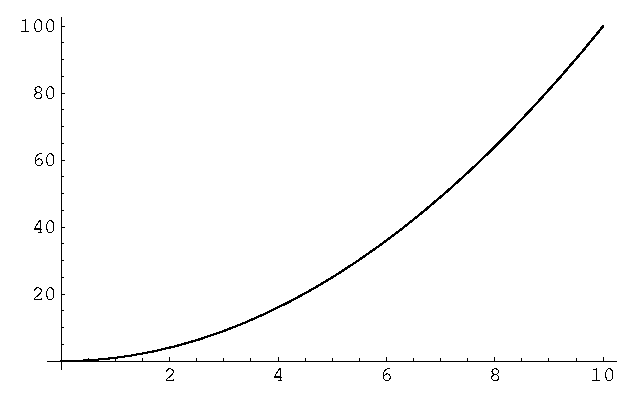
\includegraphics{plot.eps}
  \caption{%
    By default figures are not centered.
    This is a long caption to demonstrate that captions are single spaced.
  }
  \label{fi:not-centered}
\end{figure}

\Repeat{This is the second paragraph.}{10}

\begin{figure}[h]
  \centering
  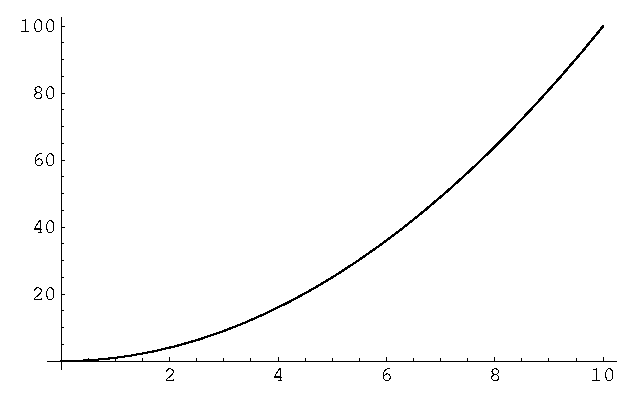
\includegraphics{plot.eps}
  \caption{Use {\tt \char'134centering\/} to center figures.}
  \label{fi:centered}
\end{figure}

\Repeat{This is the third paragraph.}{15}

\begin{figure}[h]
  \centering
  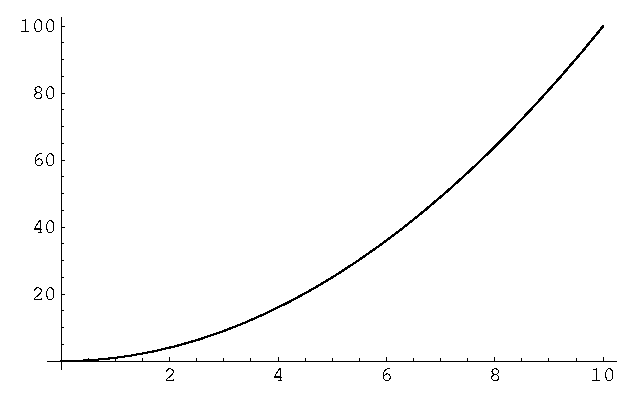
\includegraphics{plot.eps}
  \caption{This is another figuure.}
  \label{fi:another}
\end{figure}

\Repeat{This is the fourth paragraph.}{10}

\begin{figure}[h]
  \centering 
  \subfigure[First subcaption.]{\label{sf:two-parts-a}  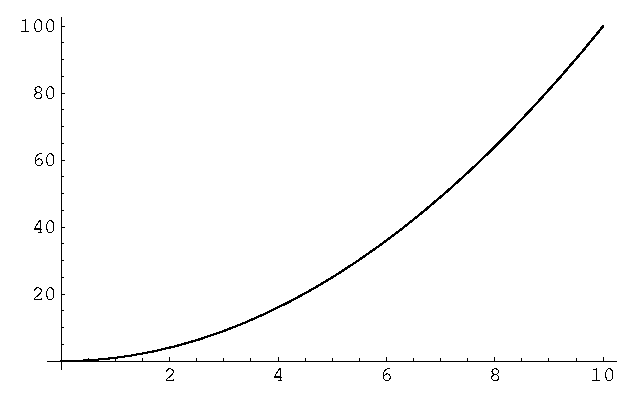
\includegraphics[width=0.3\textwidth]{plot.eps}}%
  \hskip 0.5truein
  \subfigure[Second subcaption.]{\label{sf:two-parts-b}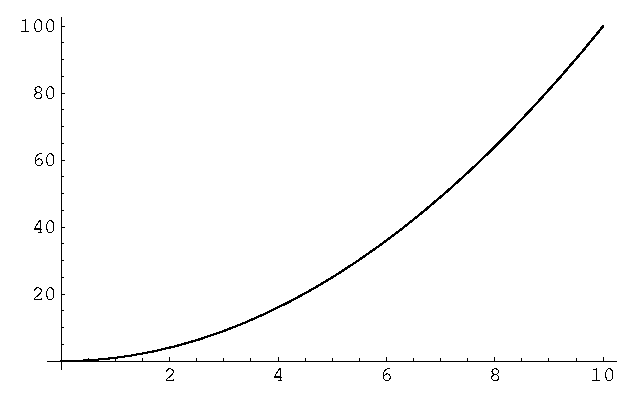
\includegraphics[width=0.3\textwidth]{plot.eps}}
  \caption{This figure has two parts.}
  \label{fi:two-parts}
\end{figure}

\Repeat{This is the fifth paragraph.}{10}

\begin{figure}[h]
  \centering
  \subfigure[First subcaption.]{\label{sf:four-parts-a}  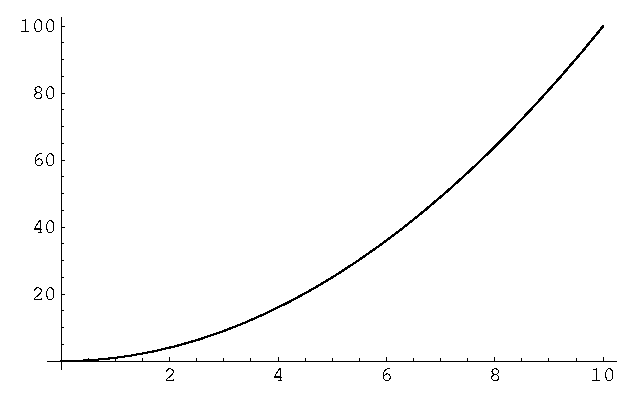
\includegraphics[width=0.3\textwidth]{plot.eps}}%
  \hskip 0.5truein
  \subfigure[Second subcaption.]{\label{sf:four-parts-b}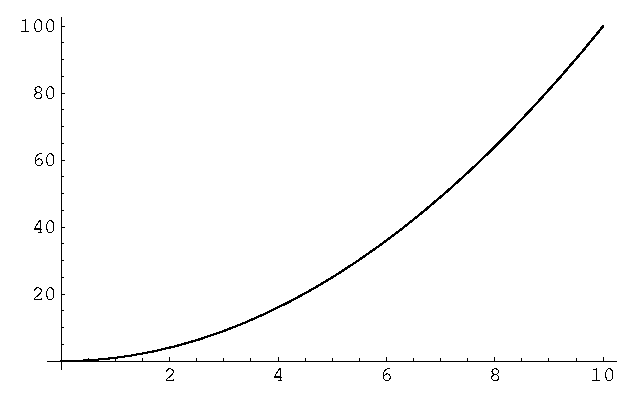
\includegraphics[width=0.3\textwidth]{plot.eps}}
  \subfigure[Third subcaption.]{\label{sf:four-parts-c}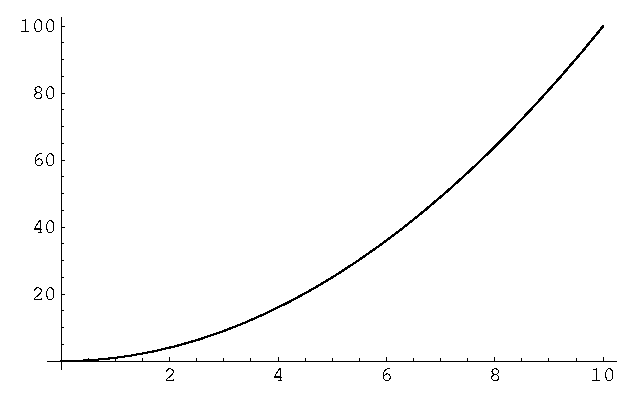
\includegraphics[width=0.3\textwidth]{plot.eps}}%
  \hskip 0.5truein
  \subfigure[Fourth subcaption.]{\label{sf:four-parts-d}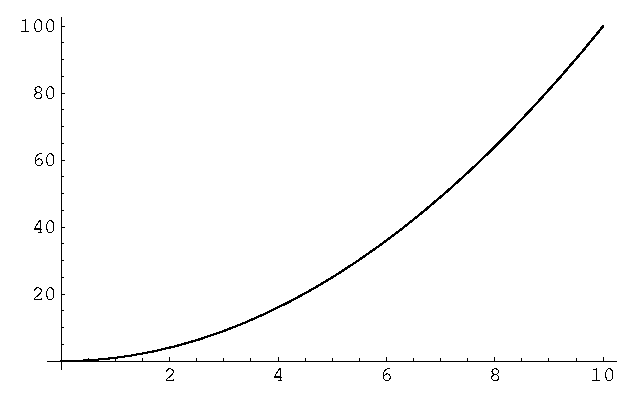
\includegraphics[width=0.3\textwidth]{plot.eps}}
  \caption{This figure has four parts.}
  \label{fi:four-parts}
\end{figure}

\Repeat{This is the sixth paragraph.}{10}

%
%  THIS FILE DOES SOME UNUSUAL THINGS TO MAKE
%  IT EASIER TO DO DEMONSTRATIONS.  IT SHOULD
%  NOT BE USED AS AN EXAMPLE OF HOW TO PREPARE
%  A FILE.  SEE THE OUTPUT OF THIS FOR LATEX
%  INPUT AND OUTPUT EXAMPLES.
%




%
%  demo-mathematics.tex  2008-12-09  Mark Senn  https://engineering.purdue.edu/~mark
%

\chapter{Demonstrate Mathematics}

    % Use single spacing.
    \Baselinestretch{1}

    % You don't normally need this.
    \mbox{}

    \begin{verbatim}
% From _More Math Into LaTeX_, 4th Edition, page 152:
%     TeX uses $$ to open and close a displayed math environment.
%     In LaTeX, this may occassionally cause problems.  Don't do it.
\[
    E = mc^2
\]
    \end{verbatim}
% From _More Math Into LaTeX_, 4th Edition, page 152:
%     TeX uses $$ to open and close a displayed math environment.
%     In LaTeX, this may occasionally cause problems.  Don't do it.
\[
    E = mc^2
\]
    \vskip\baselineskip
    \hrule
    \vskip0.5\baselineskip
    \filbreak

    \begin{verbatim}
\begin{equation}
    E = mc^2
\end{equation}
    \end{verbatim}
\begin{equation}
    E = mc^2
\end{equation}
    \vskip\baselineskip
    \hrule
    \vskip0.5\baselineskip
    \filbreak

    \begin{verbatim}
% Mydefs.tex defines \be to be \begin{equation} and
% \ee to be \end{equation}.
\be
    E = mc^2
\ee
    \end{verbatim}
% Mydefs.tex defines \be to be \begin{equation} and
% \ee to be \end{equation}.
\be
    E = mc^2
\ee
    \vskip\baselineskip
    \hrule
    \vskip0.5\baselineskip
    \filbreak

    \begin{verbatim}
\be
    x = -\frac{b}{2a} \pm \frac{\sqrt{b^2 - 4ac}}{2a}
\ee
    \end{verbatim}
\be
    x = -\frac{b}{2a} \pm \frac{\sqrt{b^2 - 4ac}}{2a}
\ee
    \vskip\baselineskip
    \hrule
    \vskip0.5\baselineskip
    \filbreak

    \begin{verbatim}
% requires \usepackage{amsmath}; use align* for no equation number
\begin{align}
    a = {}& b + c\\
    x = {}& y + z
\end{align}
    \end{verbatim}
% requires \usepackage{amsmath}; use align* for no equation number
\begin{align}
    a = {}& b + c\\
    x = {}& y + z
\end{align}
    \vskip\baselineskip
    \hrule
    \vskip0.5\baselineskip
    \filbreak

    \begin{verbatim}
\[
    Z = \left(
        \begin{array}{cc}
            a& b\\
            c& d
        \end{array}
    \right)
\]
    \end{verbatim}
\[
    Z = \left(
        \begin{array}{cc}
            a& b\\
            c& d
        \end{array}
    \right)
\]
    \vskip\baselineskip
    \hrule
    \vskip0.5\baselineskip
    \filbreak

    \begin{verbatim}
\begin{equation}
    \begin{split}
        a = {}& b + c\\
            {}& + d + e
    \end{split}      
\end{equation}
    \end{verbatim}
\begin{equation}
    \begin{split}
        a = {}& b + c\\
            {}& + d + e
    \end{split}      
\end{equation}
    \vskip\baselineskip
    \hrule
    \vskip0.5\baselineskip
    \filbreak

    \begin{verbatim}
\be
    (\cos x)^2 + (\sin x)^2 = 1
\ee
    \end{verbatim}
\be
    (\cos x)^2 + (\sin x)^2 = 1
\ee
    \vskip\baselineskip
    \hrule
    \vskip0.5\baselineskip
    \filbreak

    \begin{verbatim}
If $X = \cos x$ and $Y = \sin x$ then $X^2 + Y^2 = 1$.
    \end{verbatim}
If $X = \cos x$ and $Y = \sin x$ then $X^2 + Y^2 = 1$.
    \vskip\baselineskip
    \hrule
    \vskip0.5\baselineskip
    \filbreak

%
%  demo-multicols.tex  2007-03-19  Mark Senn  https://engineering.purdue.edu/~mark
%
%  Demonstrate multicols.
%
%  The multicols package must be loaded for this to work.
%  To load the multicols package put
%      \usepackage{multicols}
%  between the "\documentclass" and "\begin{document}" commands.
%

\chapter{Demonstrate Multicols}

% Put this amount of space between the columns.
\setlength{\columnsep}{0.5truein}

% Separate the columns with a vertical rule this wide.
\setlength{\columnseprule}{0.4pt}

\Repeat{This is one column.}{25}

\begin{multicols}{2}
\Repeat{This is two columns.}{25}
\end{multicols}

\begin{multicols}{3}
\Repeat{This is three columns.}{25}
\end{multicols}

\begin{multicols}{4}
\Repeat{This is four columns.}{25}
\end{multicols}

\begin{multicols}{5}
\Repeat{This is five columns.}{25}
\end{multicols}

%
%  demo-tables.tex  2009-09-29  Mark Senn  https://engineering.purdue.edu/~mark
%
%  Demonstrate how to do tables.
%

\chapter{Demonstrate Tables}

\begin{tabular}{ll}
    \bf Label& \bf Number\\
    ta:text-only& \ref{ta:text-only}\\
    ta:fruit&     \ref{ta:fruit}
\end{tabular}

\newlength{\ta}
\newlength{\tb}
\newlength{\tc}

\settowidth{\ta}{\vbox{\hbox{Money}\hbox{Market}}}
\settowidth{\tb}{\vbox{\hbox{Stocks}\hbox{and}\hbox{Bonds}}}
\settowidth{\tc}{\vbox{\hbox{Money}\hbox{Market}\hbox{and}\hbox{Stocks}}}

%{\renewcommand{\baselinestretch}{1}
%  \begin{table}
%    \caption{%
%      \hfil Allocation of the IRA and Keogh Wealth\hfil\break
%      \mbox{}\hfil for Investors With or Without Brokerage Accounts\hfil
%    }
%    \label{tab:ira}
%    \begin{center}
%      \begin{tabular}%
%        {%
%          |%
%          c%
%          |%
%          >{\centering\hspace{0pt}}m{\the\ta}%  Money Market
%          |%
%          c%                                    Stocks 
%          |%
%          c%                                    Bonds
%          |%
%          c%                                    Diversified
%          |%
%          >{\centering\hspace{0pt}}m{\the\tb}%  Stocks and Bonds
%          |%
%          >{\centering\hspace{0pt}}m{\the\tc}%  Money Market and Stocks
%          |%
%          c%                                    Others
%          |%
%        }
%        \hline
%        IMP&
%          Money Market&
%          Stocks&
%          Bonds&
%          Diversified&
%          Stocks and Bonds&
%          Money Market and Stocks&
%          Others\tabularnewline
%        \hline
%        1& 14.19\%& 57.71\%& 12.21\%& 4.50\%& 7.36\%& 3.04\%& 0.99\%\tabularnewline \hline
%        2& 14.08\%& 58.18\%& 12.32\%& 4.44\%& 7.30\%& 2.80\%& 0.88\%\tabularnewline \hline
%        3 &14.26\%& 58.09\%& 12.27\%& 4.50\%& 7.19\%& 2.75\%& 0.94\%\tabularnewline \hline
%        4 &13.94\%& 58.11\%& 12.14\%& 4.78\%& 7.35\%& 2.68\%& 0.99\%\tabularnewline \hline
%        5 &13.92\%& 58.13\%& 11.93\%& 4.56\%& 7.60\%& 2.98\%& 0.88\%\tabularnewline \hline
%      \end{tabular}
%    \end{center}
%    This table presents the allocations of the wealth in the IRA
%    and Keogh accounts in various asset classes.
%    Results from each set of imputed data are presented here.
%    The first column lists the number of the imputations,
%    and rest of the columns lists various allocations.
%    Entrees under each asset class show the percentage of investors
%    who have most of their IRA
%    and Keogh wealth invested in that particular asset class.
%    The asset class Diversified
%    includes stocks,
%    bonds,
%    and money market investments.
%    The asset class Others
%    include investments in various life insurance products,
%    annuities,
%    real estate, etc.
%    \medskip
%    \footnotesize SOURCE: Survey of Consumer Finances,
%    2001,
%    Federal Reserve Board,
%    USA.\par
%  \end{table}
%}

\begin{table}
    This table contains only text.
    Let's cite Lamport's book here: \cite{Lamport:1994}.
    \caption{%
        This is the caption.
        Let's cite Lamport's book again here: \cite{Lamport:1994}.%
    }
    \label{ta:text-only}
\end{table}

\begin{table}
    % \halign{...} is more flexible than \begin{table}...\end{table}.
    \hbox to \textwidth{%
         \hfill
        \vbox{\halign{
            \strut #&            % 0. \strut
            #\hfil\qquad&        % 1. left
            \hfil #\hfil\qquad&  % 2. center
            \hfil #\cr           % 3. right
            %
            & apple& banana& cherry\cite{Lamport:1994}\cr
            & aardvark& boa constrictor& coyote\cr
        }}
        \hfill
    }
    \caption[short caption for table of contents]{%
        This is a really long and boring caption.
        It goes on and on as if it thinks what it says is important.
        Here is some more of it.
        The citation for ``Lamport::1994'' is ``\cite{Lamport:1994}''.%
    }
    \label{ta:fruit}
\end{table}

% This is loosely based on page 106 of _A Guide to LaTeX_, third edition,
% by Helmut Kopka and Patrick W. Daly.
%\begin{longtable}{|l|l|}
%  \caption{2.2 ``State'' Abbreviations}\\
%  \hline
%  ``State''& Abbreviation\\
%  \hline \endfirsthead
%  \caption[]{\emph{continued}}\\
%  \hline
%  ``State''& Abbreviation\\
%  \hline \endhead
%  \hline
%  \multicolumn{2}{r}{\emph{continued on next page}}
%  \endfoot
%  \hline\endlastfoot
%  Alabama& AL\\
%  Alaska& AK\\
%  American Samoa& AS\\
%  Arizona& AZ\\
%  Arkansas& AR\\
%  Armed Forces Europe& AE\\
%  Armed Forces Pacific& AP\\
%  Armed Forces the Americas& AA\\
%  California& CA\\
%  Colorado& CO\\
%  Connecticut& CT\\
%  Delaware& DE\\
%  District of Columbia& DC\\
%  Federated States of Micronesia& FM\\
%  Florida& FL\\
%  Georgia& GA\\
%  Guam& GU\\
%  Hawaii& HI\\
%  Idaho& ID\\
%  Illinois& IL\\
%  Indiana& IN\\
%  Iowa& IA\\
%  Kansas& KS\\
%  Kentucky& KY\\
%  Louisiana& LA\\
%  Maine& ME\\
%  Marshall Islands& MH\\
%  Maryland& MD\\
%  Massachusetts& MA\\
%  Michigan& MI\\
%  Mississippi& MS\\
%  Missouri& MO\\
%  Montana& MT\\
%  N Minnesota
%  Nebraska& NE\\
%  Nevada& NV\\
%  New Hampshire& NH\\
%  New Jersey& NJ\\
%  New Mexico& NM\\
%  New York& NY\\
%  North Carolina& NC\\
%  North Dakota& ND\\
%  Northern Mariana Islands& MP\\
%  Ohio& OH\\
%  Oklahoma& OK\\
%  Oregon& OR\\
%  Pennsylvania& PA\\
%  Puerto Rico& PR\\
%  Rhode Island& RI\\
%  South Carolina& SC\\
%  South Dakota& SD\\
%  Tennessee& TN\\
%  Texas& TX\\
%  Utah& UT\\
%  Vermont& VT\\
%  Virgin Islands, U.S.& VI\\
%  Virginia& VA\\
%  Washington& WA\\
%  West Virginia& WV\\
%  Wisconsin& WI\\
%  Wyoming& WY\\
%\end{longtable}

\newcommand{\cbackslash}{\char'134}
\newcommand{\copencurly}{\char'173}
\newcommand{\cclosecurly}{\char'175}

\newlength{\twidth}
\newlength{\theight}

\setlength{\twidth}{\textwidth}
\setlength{\theight}{\textheight}

\begin{sidewaystable}
    % The following two lines compensate for what I think is a bug.
    \setlength{\textwidth}{\theight}
    \setlength{\textheight}{\twidth}
    \caption{%
        2.3 sidewaystable mode
        {\tt\cbackslash begin\copencurly table\cclosecurly\/}%
        \ldots
        {\tt\cbackslash end\copencurly table\cclosecurly\/} table%
    }
    \hbox to \textwidth{
        \hfill
        \begin{tabular}{lcr}
            apple& banana& cherry\\
            aardvark& boa constrictor& coyote\\
        \end{tabular}
        \hfill
    }
\end{sidewaystable}

\begin{sidewaystable}
    % The following two lines compensate for what I think is a bug.
    \setlength{\textwidth}{\theight}
    \setlength{\textheight}{\twidth}
    \caption{%
        2.4 sidewaystable mode
        {\tt\cbackslash halign\copencurly ...\cclosecurly\/} table%
    }
    \hbox to \textwidth{%
        \hfill
        \vbox{\halign{
            \strut #&            % 0. \strut
            #\hfil\qquad&        % 1. left
            \hfil #\hfil\qquad&  % 2. center
            \hfil #\cr           % 3. right
            %
            & apple& banana& cherry\cr
            & aardvark& boa constrictor& coyote\cr
        }}
        \hfill
    }
\end{sidewaystable}

\begin{table}
    \begin{tabular}{lcr}
        apple& banana& cherry\\
        aardvark& boa constrictor& coyote\\
        apple& banana& cherry\\
        aardvark& boa constrictor& coyote\\
        apple& banana& cherry\\
        aardvark& boa constrictor& coyote\\
        apple& banana& cherry\\
        aardvark& boa constrictor& coyote\\
        apple& banana& cherry\\
        aardvark& boa constrictor& coyote\\
        apple& banana& cherry\\
        aardvark& boa constrictor& coyote\\
        apple& banana& cherry\\
        aardvark& boa constrictor& coyote\\
        apple& banana& cherry\\
        aardvark& boa constrictor& coyote\\
    \end{tabular}
    \caption{2.5 left hand table}
\end{table}

\begin{table}
    \begin{tabular}{lcr}
        apple& banana& cherry\\
        aardvark& boa constrictor& coyote\\
    \end{tabular}
    \caption{2.6 left hand table}
\end{table}

\begin{sidewaystable}
    % The following two lines compensate for what I think is a bug.
    \setlength{\textwidth}{\theight}
    \setlength{\textheight}{\twidth}
    \caption{%
        2.7 sidewaystable mode
        {\tt\cbackslash begin\copencurly table\cclosecurly\/}%
        \ldots
        {\tt\cbackslash end\copencurly table\cclosecurly\/} table%
    }
    \hbox to \textwidth{%
        \hfill
        \begin{tabular}{lcr}
            apple& banana& cherry\\
            aardvark& boa constrictor& coyote\\
        \end{tabular}
        \hfill
    }
\end{sidewaystable}

%\newlength{\ta}
%\settowidth{\ta}{\vbox{\hbox{Money}\hbox{Market}}}
%\newlength{\tb}
%\settowidth{\tb}{\vbox{\hbox{Stocks}\hbox{and}\hbox{Bonds}}}
%\newlength{\tc}
%\settowidth{\tc}{\vbox{\hbox{Money}\hbox{Market}\hbox{and}\hbox{Stocks}}}
%
%  {\renewcommand{\baselinestretch}{1}
%\begin{table}
%  \caption{\hfil Allocation of the IRA and Keogh Wealth\hfil\break\mbox{}\hfil for Investors With or Without Brokerage Accounts\hfil}
%  \label{tab:ira}
%  \begin{center}
%    \begin{tabular}%
%      {%
%        |%
%        c%
%        |%
%        >{\centering\hspace{0pt}}m{\the\ta}%  Money Market
%        |%
%        c%                                    Stocks 
%        |%
%        c%                                    Bonds
%        |%
%        c%                                    Diversified
%        |%
%        >{\centering\hspace{0pt}}m{\the\tb}%  Stocks and Bonds
%        |%
%        >{\centering\hspace{0pt}}m{\the\tc}%  Money Market and Stocks
%        |%
%        c%                                    Others
%        |%
%      }
%      \hline
%      IMP&
%        Money Market&
%        Stocks&
%        Bonds&
%        Diversified&
%        Stocks and Bonds&
%        Money Market and Stocks&
%        Others\tabularnewline
%      \hline
%      1& 14.19\%& 57.71\%& 12.21\%& 4.50\%& 7.36\%& 3.04\%& 0.99\%\tabularnewline \hline
%      2& 14.08\%& 58.18\%& 12.32\%& 4.44\%& 7.30\%& 2.80\%& 0.88\%\tabularnewline \hline
%      3 &14.26\%& 58.09\%& 12.27\%& 4.50\%& 7.19\%& 2.75\%& 0.94\%\tabularnewline \hline
%      4 &13.94\%& 58.11\%& 12.14\%& 4.78\%& 7.35\%& 2.68\%& 0.99\%\tabularnewline \hline
%      5 &13.92\%& 58.13\%& 11.93\%& 4.56\%& 7.60\%& 2.98\%& 0.88\%\tabularnewline \hline
%    \end{tabular}
%  \end{center}
%  This table presents the allocations of the wealth in the IRA
%  and Keogh accounts in various asset classes.
%  Results from each set of imputed data are presented here.
%  The first column lists the number of the imputations,
%  and rest of the columns lists various allocations.
%  Entrees under each asset class show the percentage of investors
%  who have most of their IRA
%  and Keogh wealth invested in that particular asset class.
%  The asset class Diversified
%  includes stocks,
%  bonds,
%  and money market investments.
%  The asset class Others
%  include investments in various life insurance products,
%  annuities,
%  real estate, etc.
%  \medskip
%  \footnotesize SOURCE: Survey of Consumer Finances,
%  2001,
%  Federal Reserve Board,
%  USA.\par
%\end{table}
%  }

\begin{table}
    \caption{Presidents}
    \begin{center}
        \begin{tabular}{cl}
            \#& Name\\
            1&  George Washington\\
            2&  John Adams\\
            3&  Thomas Jefferson\\
        \end{tabular}
    \end{center}
\end{table}

\begin{table}
    \caption{Presidents with horizontal and vertical lines}
    \begin{center}
        \begin{tabular}{|c|l|}
            \hline
            \#& Name\\
            \hline
            1&  George Washington\\
            \hline
            2&  John Adams\\
            \hline
            3&  Thomas Jefferson\\
            \hline
        \end{tabular}
    \end{center}
\end{table}

%
%  demo-text.tex  2007-07-17  Mark Senn  https://engineering.purdue.edu/~mark
%

\chapter{Demonstrate Text}

% Use single spacing.
\Baselinestretch{1}

% You don't normally need this.
\mbox{}


%\vbox{
\begin{verbatim}
This is a sentence.
This is a sentence.
This is a sentence.
This is a sentence.
This is a sentence.

This is a sentence.
This is a sentence.
This is a sentence.
This is a sentence.
This is a sentence.
\end{verbatim}
This is a sentence.
This is a sentence.
This is a sentence.
This is a sentence.
This is a sentence.

This is a sentence.
This is a sentence.
This is a sentence.
This is a sentence.
This is a sentence.
\vskip\baselineskip
\hrule
%}
\vskip0.5\baselineskip
\filbreak

%\vbox{
\begin{verbatim}
From \verb+http://www.biblegateway.com/passage/?book_id=1&chapter=1&version=50+:

\begin{quote}
    1 In the beginning God created the heavens and the earth.
    2 The earth was without form,
    and void;
    and darkness was on the face of the deep.
    And the Spirit of God was hovering over the face of the waters.

    3 Then God said,``Let there be light'';
    and there was light.
    4 And God saw the light,
    that it was good;
    and God divided the light from the darkness.
    5 God called the light Day,
    and the darkness He called Night.
    So the evening and the morning were the first day. 
\end{quote}
\end{verbatim}
From \verb+http://www.biblegateway.com/passage/?book_id=1&chapter=1&version=50+:

\begin{quote}
    1 In the beginning God created the heavens and the earth.
    2 The earth was without form,
    and void;
    and darkness was on the face of the deep.
    And the Spirit of God was hovering over the face of the waters.

    3 Then God said,``Let there be light'';
    and there was light.
    4 And God saw the light,
    that it was good;
    and God divided the light from the darkness.
    5 God called the light Day,
    and the darkness He called Night.
    So the evening and the morning were the first day. 
\end{quote}
\vskip\baselineskip
\hrule
%}
\vskip0.5\baselineskip
\filbreak

%\vbox{
\begin{verbatim}
\begin{description}
    \item[apple]
        A red fruit.
    \item[banana]
        A yellow fruit.
        This sentence is to make the entry longer so you can see what happens.
        This sentence is to make the entry longer so you can see what happens.
    \item[cherry]
        A red friut.
\end{description}
\end{verbatim}
\begin{description}
    \item[apple]
        A red fruit.
    \item[banana]
        A yellow fruit.
        This sentence is to make the entry longer so you can see what happens.
        This sentence is to make the entry longer so you can see what happens.
    \item[cherry]
        A red friut.
\end{description}
\vskip\baselineskip
\hrule
%}
\vskip0.5\baselineskip
\filbreak

%\vbox{
\begin{verbatim}
\begin{enumerate}
    \item apple
    \item banana
        This sentence is to make the entry longer so you can see what happens.
        This sentence is to make the entry longer so you can see what happens.
    \item cherry
\end{enumerate}
\end{verbatim}
\begin{enumerate}
    \item apple
    \item banana
        This sentence is to make the entry longer so you can see what happens.
        This sentence is to make the entry longer so you can see what happens.
    \item cherry
\end{enumerate}
\vskip\baselineskip
\hrule
%}
\vskip0.5\baselineskip
\filbreak


%\vbox{
\begin{verbatim}
\begin{itemize}
    \item apple
    \item banana
        This sentence is to make the entry longer so you can see what happens.
        This sentence is to make the entry longer so you can see what happens.
    \item cherry
\end{itemize}
\end{verbatim}
\begin{itemize}
    \item apple
    \item banana
        This sentence is to make the entry longer so you can see what happens.
        This sentence is to make the entry longer so you can see what happens.
    \item cherry
\end{itemize}
\vskip\baselineskip
\hrule
%}
\vskip0.5\baselineskip
\filbreak


% Bibliography is required if you consulted any outside references.
% Reference: TM 32.
%
%  bibliography.tex  2011-07-19  Mark Senn  https://engineering.purdue.edu/~mark
%
%  This is the bibliography for the thesis.
%

% IF YOU USE BIBTEX USE THE FOLLOWING LINE:
\bibliography{all}

% If BibTeX produces a .bbl file that is close to what you want but
% not exactly right you may want to include the contents of the .bbl
% file below and use the instructions immediately below.  If you do
% this you'll want to do it after you've cited all your references
% and are running LaTeX on the final copy of your thesis.  I recommend
% running LaTeX three times after changing this file like you'd like
% it.

% OTHERWISE (YOU ARE NOT USING BIBTEX), USE THE FOLLOWING LINES:
% Format the bibliography items like your school or department wants.
%\begin{thebibliography}{}
%
%\bibitem{Kopka:2004}
%Kopka H. and Daly P. W.,
%\emph{A Guide to \LaTeX:
%    Document Preparation for Beginners and Advanced Users}.
%
%\bibitem{Lamport:1994}
%Lamport L.,
%\emph{\LaTeX: A Document Preparation System}.
%
%\bibitem{Mittelbach:2004}
%Mittelbach F. and Goossens M.,
%\emph{The \LaTeX\ Companion}.
%
%\end{thebibliography}


% Notes and footnotes are optional.
% Reference: TM 34.
% I have not implemented this yet.  Mark Senn 2002-06-03
%%\include{notes}

% A vita is optional for masters theses
% and required for doctoral dissertations.
% Reference: TM 13.
% CHANGE NEXT LINE?
%
%  vita.tex  2012-01-18  Mark Senn  https://engineering.purdue.edu/~mark
%
%  A vita is optional for masters theses
%  and required for doctoral dissertations.
%

\begin{vita}
  The remainder
  of this page was taken from page 13
  of the Grad School's thesis manual.

  Ph.D.~candidates are required to include a vita in their dissertation;
  however,
  this is optional for master's candidates.
  The vita is normally the last major division
  of the dissertation
  (unless followed by a publication)
  and should be separated from the preceding material
  by a cover sheet that is neither numbered nor counted.
  The content of this section will be largely driven
  by departmental requirements;
  in some cases,
  you may be asked to provide a curriculum vitae,
  detailing your professional and academic resume.
\end{vita}


\end{document}

% LaTeX won't read after the \end{document} command.
% You can put notes to yourself or LaTeX input not
% ready for use here if you'd like.
